\documentclass[landscape,a0paper,fontscale=0.292]{baposter}

\usepackage[vlined]{algorithm2e}
\usepackage{times}
\usepackage{calc}
\usepackage{url}
\usepackage{graphicx}
\usepackage{amsmath}
\usepackage{amssymb}
\usepackage{relsize}
\usepackage{multirow}
\usepackage{booktabs}
\usepackage{makecell}
\usepackage{threeparttable}
\usepackage{subfig}
\usepackage{graphbox}

\usepackage{multicol}
\usepackage[T1]{fontenc}
\usepackage{ae}
\usepackage{enumitem}

\usepackage{colortbl}
\usepackage{xcolor}

\definecolor{darkcyan}{HTML}{bfd8d9}
\definecolor{ctitle}{HTML}{0c3436}

\usepackage[pagebackref=true,breaklinks=true,colorlinks=true,bookmarks=false,linkcolor={red!50!black},urlcolor={magenta},citecolor={green!50!black}]{hyperref} 

\setlist[itemize]{leftmargin=*,nosep}
    \setlength{\columnsep}{0.7em}
    \setlength{\columnseprule}{0mm}

\setlist[enumerate]{leftmargin=2.5em,nosep}
    \setlength{\columnsep}{1.0em}
    \setlength{\columnseprule}{0mm}

% %%%%%%%%%%%%%%%%%%%%%%%%%%%%%%%%%%%%%%%%%%%%%%%%%%%%%%%%%%%%%%%%%%%%%%%%%%%%%%%%
% % Save space in lists. Use this after the opening of the list
% %%%%%%%%%%%%%%%%%%%%%%%%%%%%%%%%%%%%%%%%%%%%%%%%%%%%%%%%%%%%%%%%%%%%%%%%%%%%%%%%
% \newcommand{\compresslist}{%
% \setlength{\itemsep}{0pt}%
% \setlength{\itemsep}{0pt}%
% \setlength{\parskip}{0pt}%
% \setlength{\parsep}{0pt}%
% }
\renewcommand{\rmdefault}{ptm} % Arial
\renewcommand{\sfdefault}{ptm} % Arial

\newcommand{\lout}{\hat{I}}
\newcommand{\lin}{L_i}
\newcommand{\din}{\boldsymbol{w}_i}
\newcommand{\dout}{\boldsymbol{w}_o}
\newcommand{\normal}{\boldsymbol{n}}
\newcommand{\brdf}{f_r}
\newcommand{\vmlp}{f_v}
\newcommand{\point}{\boldsymbol{x}}
%%%%%%%%%%%%%%%%%%%%%%%%%%%%%%%%%%%%%%%%%%%%%%%%%%%%%%%%%%%%%%%%%%%%%%%%%%%%%
%% Begin of Document
%%%%%%%%%%%%%%%%%%%%%%%%%%%%%%%%%%%%%%%%%%%%%%%%%%%%%%%%%%%%%%%%%%%%%%%%%%%%%
\begin{document}
%%%%%%%%%%%%%%%%%%%%%%%%%%%%%%%%%%%%%%%%%%%%%%%%%%%%%%%%%%%%%%%%%%%%%%%%%%%%%
%% Here starts the poster
%%---------------------------------------------------------------------------
%% Format it to your taste with the options
%%%%%%%%%%%%%%%%%%%%%%%%%%%%%%%%%%%%%%%%%%%%%%%%%%%%%%%%%%%%%%%%%%%%%%%%%%%%%
\begin{poster}{
    % Show grid to help with alignment
    grid=false,
    columns=6,
    % Column spacing
    colspacing=0.7em,
    % Color style
    headerColorOne=darkcyan,
    borderColor=darkcyan,
    % Format of textbox
    textborder=faded,
    % Format of text header
    headerborder=open,
    headershape=roundedright,
    headershade=plain,
    background=none,
    bgColorOne=cyan!10!white,
    headerheight=0.13\textheight
}
% Eye Catcher
{
    \raisebox{0.07\height}{
\includegraphics[height=0.0445\linewidth]{logo/HKU}}
    \makebox[0.005\textwidth]{} 
    \raisebox{0.07\height}{
\includegraphics[height=0.0445\linewidth]{logo/cuhksz}}
    \makebox[0.005\textwidth]{} 
    \raisebox{0.07\height}{
\includegraphics[height=0.0445\linewidth]{logo/NTU}}
    \makebox[0.005\textwidth]{} 
    \raisebox{0.07\height}{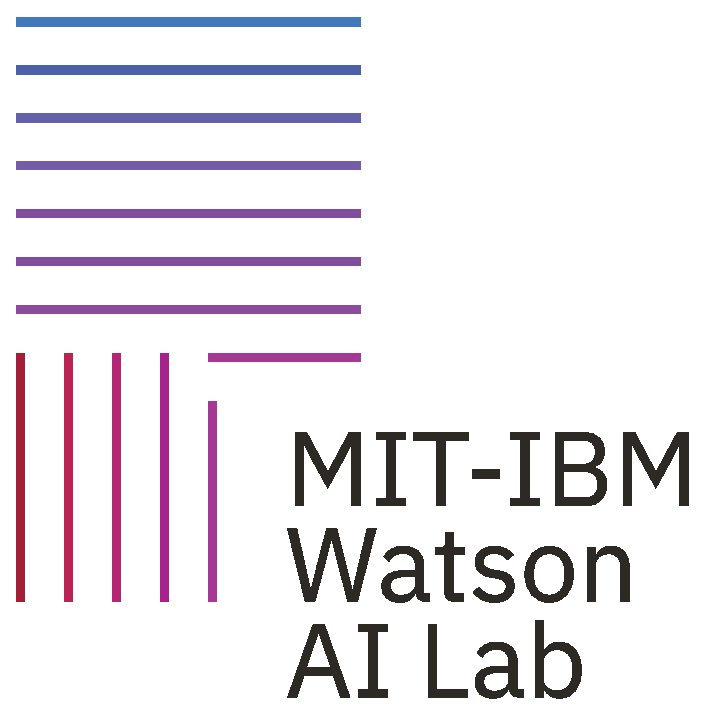
\includegraphics[height=0.0445\linewidth]{logo/MIT-IBM}}
}
% Title
{
    \\[0.3em]\sc\huge\bf \textcolor{ctitle}{PS-NeRF}: Neural Inverse Rendering for Multi-view Photometric Stereo
}
% Authors
{
    \vspace{0.3em} Wenqi Yang$^1$ \enspace Guanying Chen$^2$ \enspace Chaofeng Chen$^3$ \enspace Zhenfang Chen$^4$ \enspace Kwan-Yee K. Wong$^1$ \\[0.2em]
    {$^1$The University of Hong Kong \enspace$^2$FNii and SSE, CUHK-Shenzhen \\[0.1em] $^3$Nanyang Technological University \enspace$^4$MIT-IBM Watson AI Lab}
}
% University logo
{
    \begin{tabular}{c}
        \raisebox{-1.0\height}{
\includegraphics[align=c,width=0.1\linewidth]{logo/ECCV}}\\
        \raisebox{-0.7\height}{
        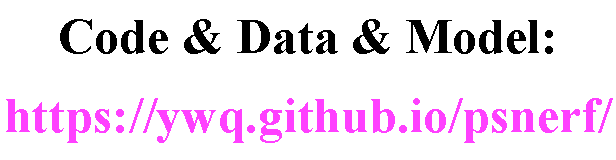
\includegraphics[align=c,width=0.095\linewidth]{logo/link.pdf}\hspace{0.002\linewidth}
        
\includegraphics[align=c,height=0.035\linewidth]{logo/qr_code.png}}
    \end{tabular}
}

%%%%%%%%%%%%%%%%%%%%%%%%%%%%%%%%%%%%%%%%%%%%%%%%%%%%%%%%%%%%%%%%%%%%%%%%%%%%%%
%%% Now define the boxes that make up the poster
%%%---------------------------------------------------------------------------
%%% Each box has a name and can be placed absolutely or relatively.
%%% The only inconvenience is that you can only specify a relative position 
%%% towards an already declared box. So if you have a box attached to the 
%%% bottom, one to the top and a third one which should be inbetween, you 
%%% have to specify the top and bottom boxes before you specify the middle 
%%% box.
%%%%%%%%%%%%%%%%%%%%%%%%%%%%%%%%%%%%%%%%%%%%%%%%%%%%%%%%%%%%%%%%%%%%%%%%%%%%%%

%%%%%%%%%%%%%%%%%%%%%%%%%%%%%%%%%%%%%%%%%%%%%%%%%%%%%%%%%%%%%%%%%%%%%%%%%%%%%%
\headerbox{\bf\color{ctitle} Problem and Contribution}{name=contribution,column=0,row=0,span=6}{
    \begin{minipage}[c]{0.32\textwidth}
        \textbf{\color{ctitle}Idea:}  \\
        Given multi-view and multi-light images of an object taken from M sparse views, PS-NeRF simultaneously reconstructs its shape, materials, and lights.
        \begin{center}
            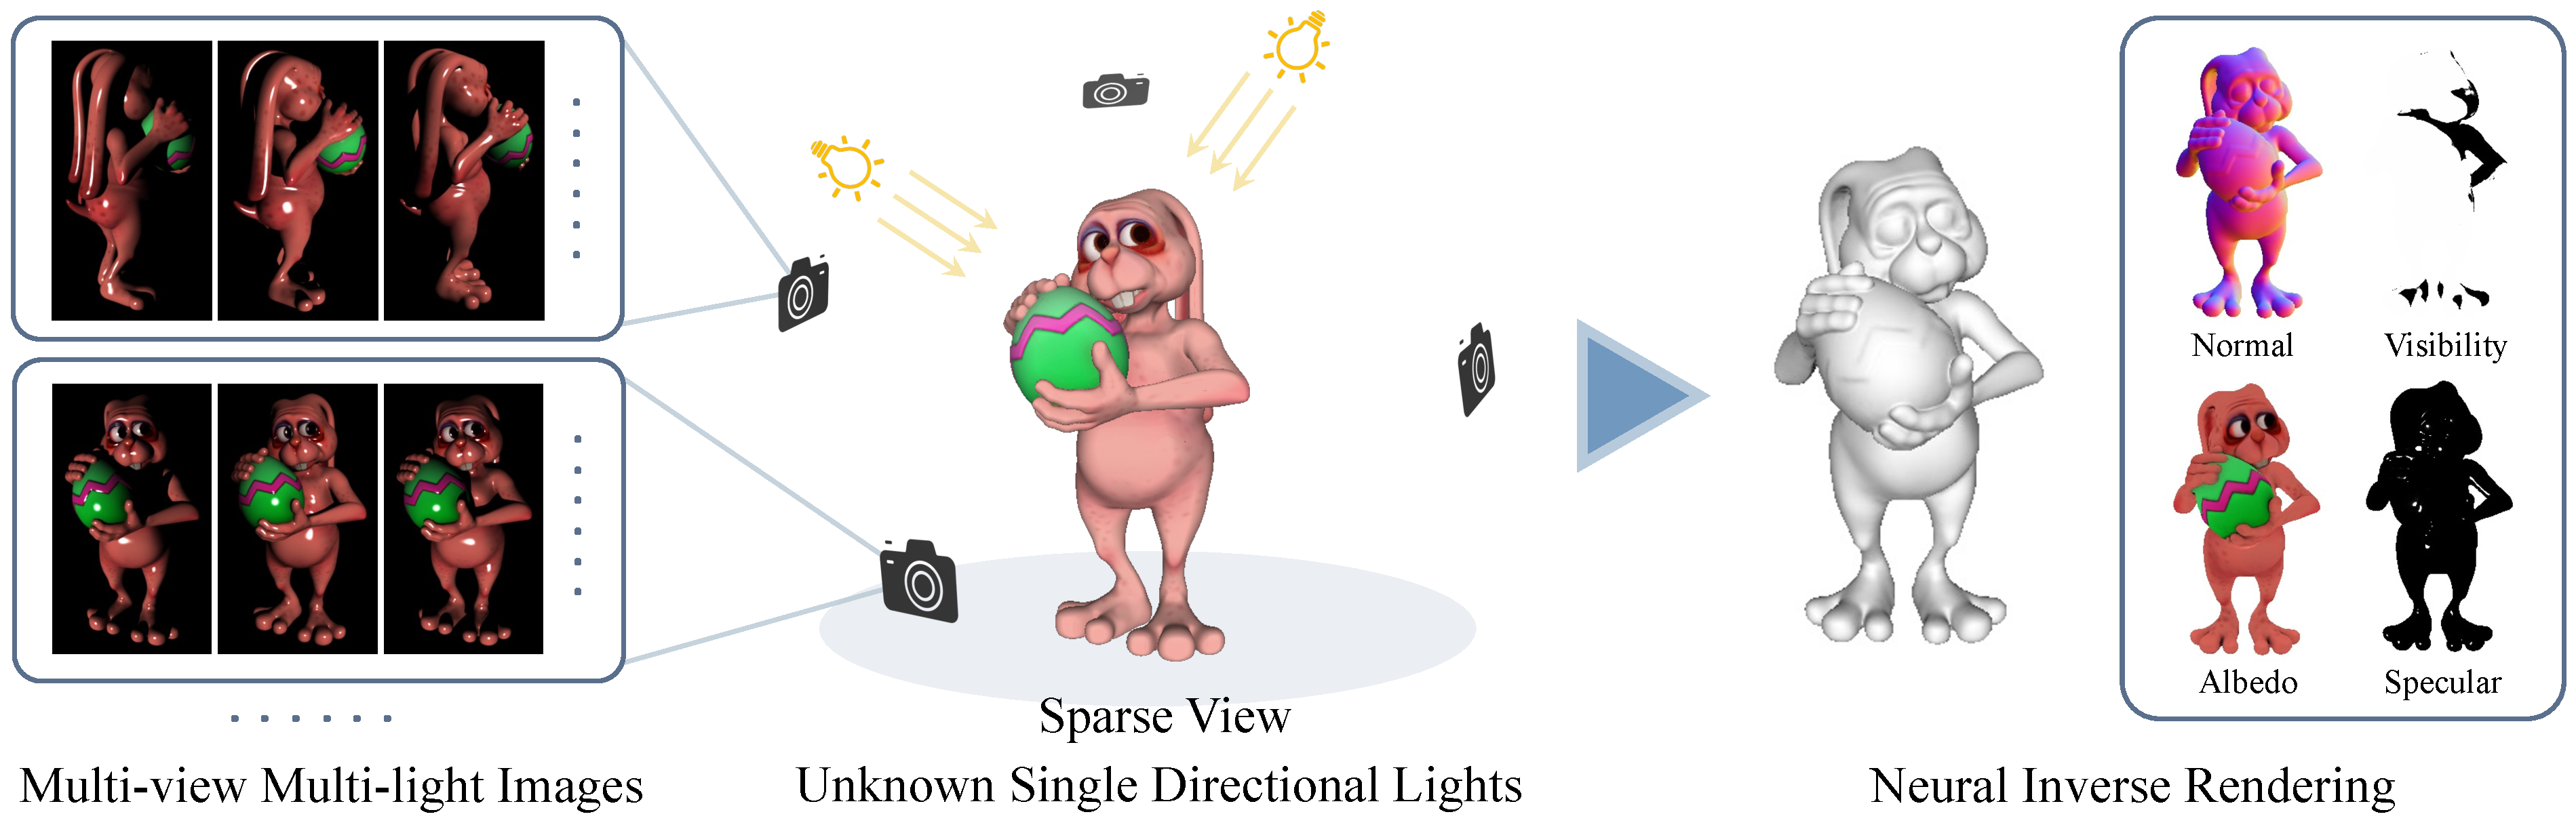
\includegraphics[width=0.95\textwidth]{images/teaser_v2}
        \end{center}
    \end{minipage}\hfill
    \begin{minipage}[c]{0.2\textwidth}
        \textbf{\color{ctitle}Contributions:}
        \begin{itemize}
            \item A neural inverse rendering method for multi-view photometric stereo  which jointly optimizes shape, BRDFs, and lights based on a shadow-aware differentiable rendering layer.
            \item We propose to regularize the implicit surface with normals estimated from multi-light images, which  significantly improves surface reconstruction, especially for sparse input views (e.g., 5 views).
            \item Our method achieves state-of-the-art results. 
        \end{itemize}  
        \vspace{0.5em}
    \end{minipage}\hfill
    \begin{minipage}[c]{0.45\textwidth}
        \textbf{\color{ctitle}Comparison with Existing Neural Rendering Methods:} 
        \vspace{-0.5em}
        \begin{center}
            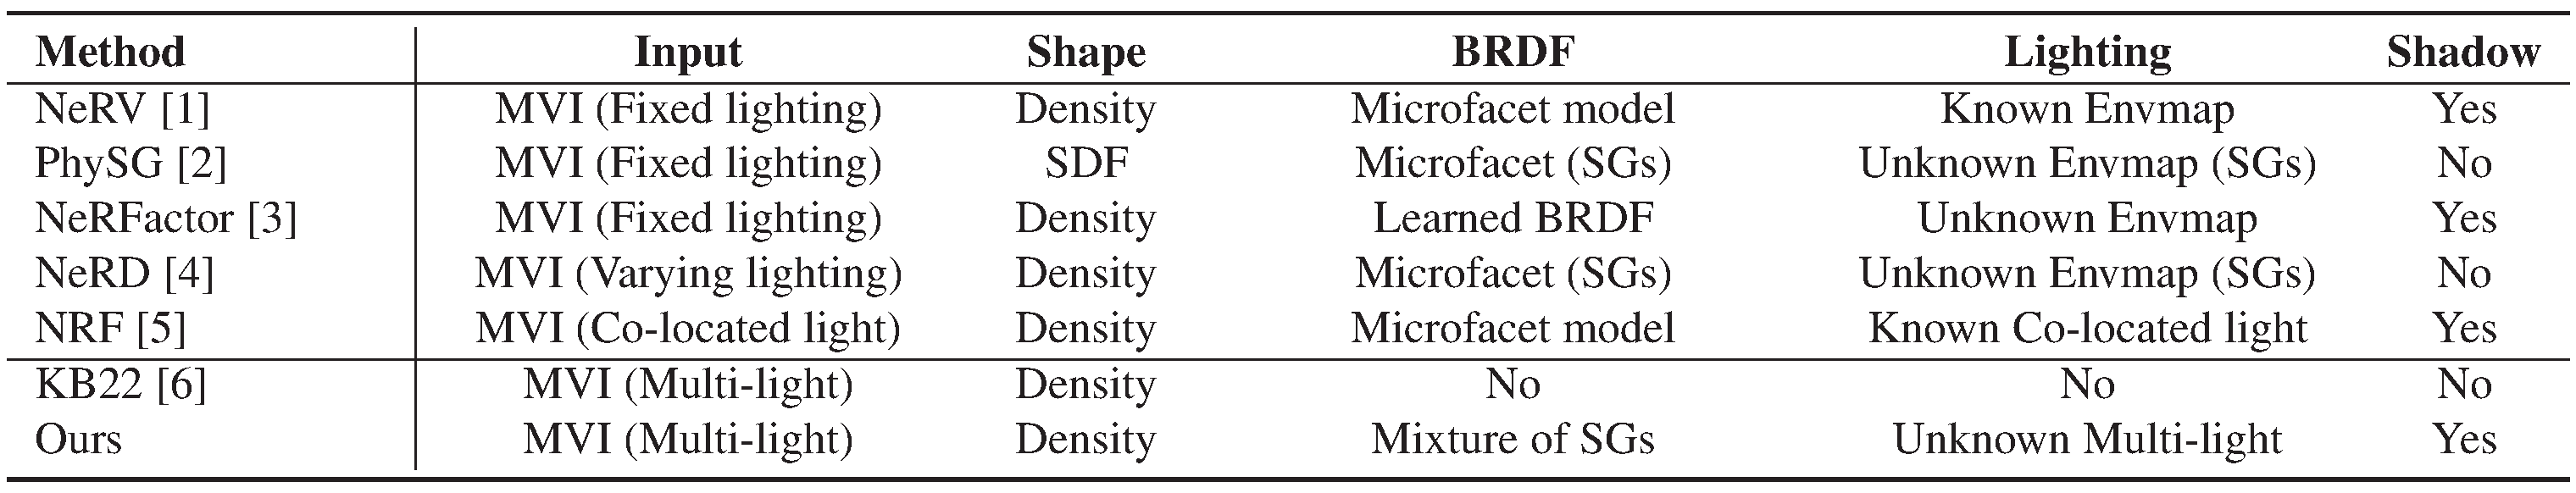
\includegraphics[width=\textwidth]{images/table_relatedwork.pdf}
        \end{center}
        \vspace{-1em}
        \begin{itemize}
            \item Our method is the only one that explicitly models surface reflectances and lights under a MVPS setup.
            \item Our results demonstrate that incorporating multi-light information appropriately can produce a far more accurate shape reconstruction.
        \end{itemize}
         
    \end{minipage}
}

\headerbox{\bf\color{ctitle} Method}{name=method,column=0,below=contribution,span=2}{
    \textbf{\color{ctitle}Overview:} \\
    Inspired by the recent success of neural radiance field [9] for 3D scene representation, we represent the object shape with a density field. Our method consists of two stages to make full use of multi-view multi-light images. \\
    \vspace{-1.5em}
    \begin{center}
        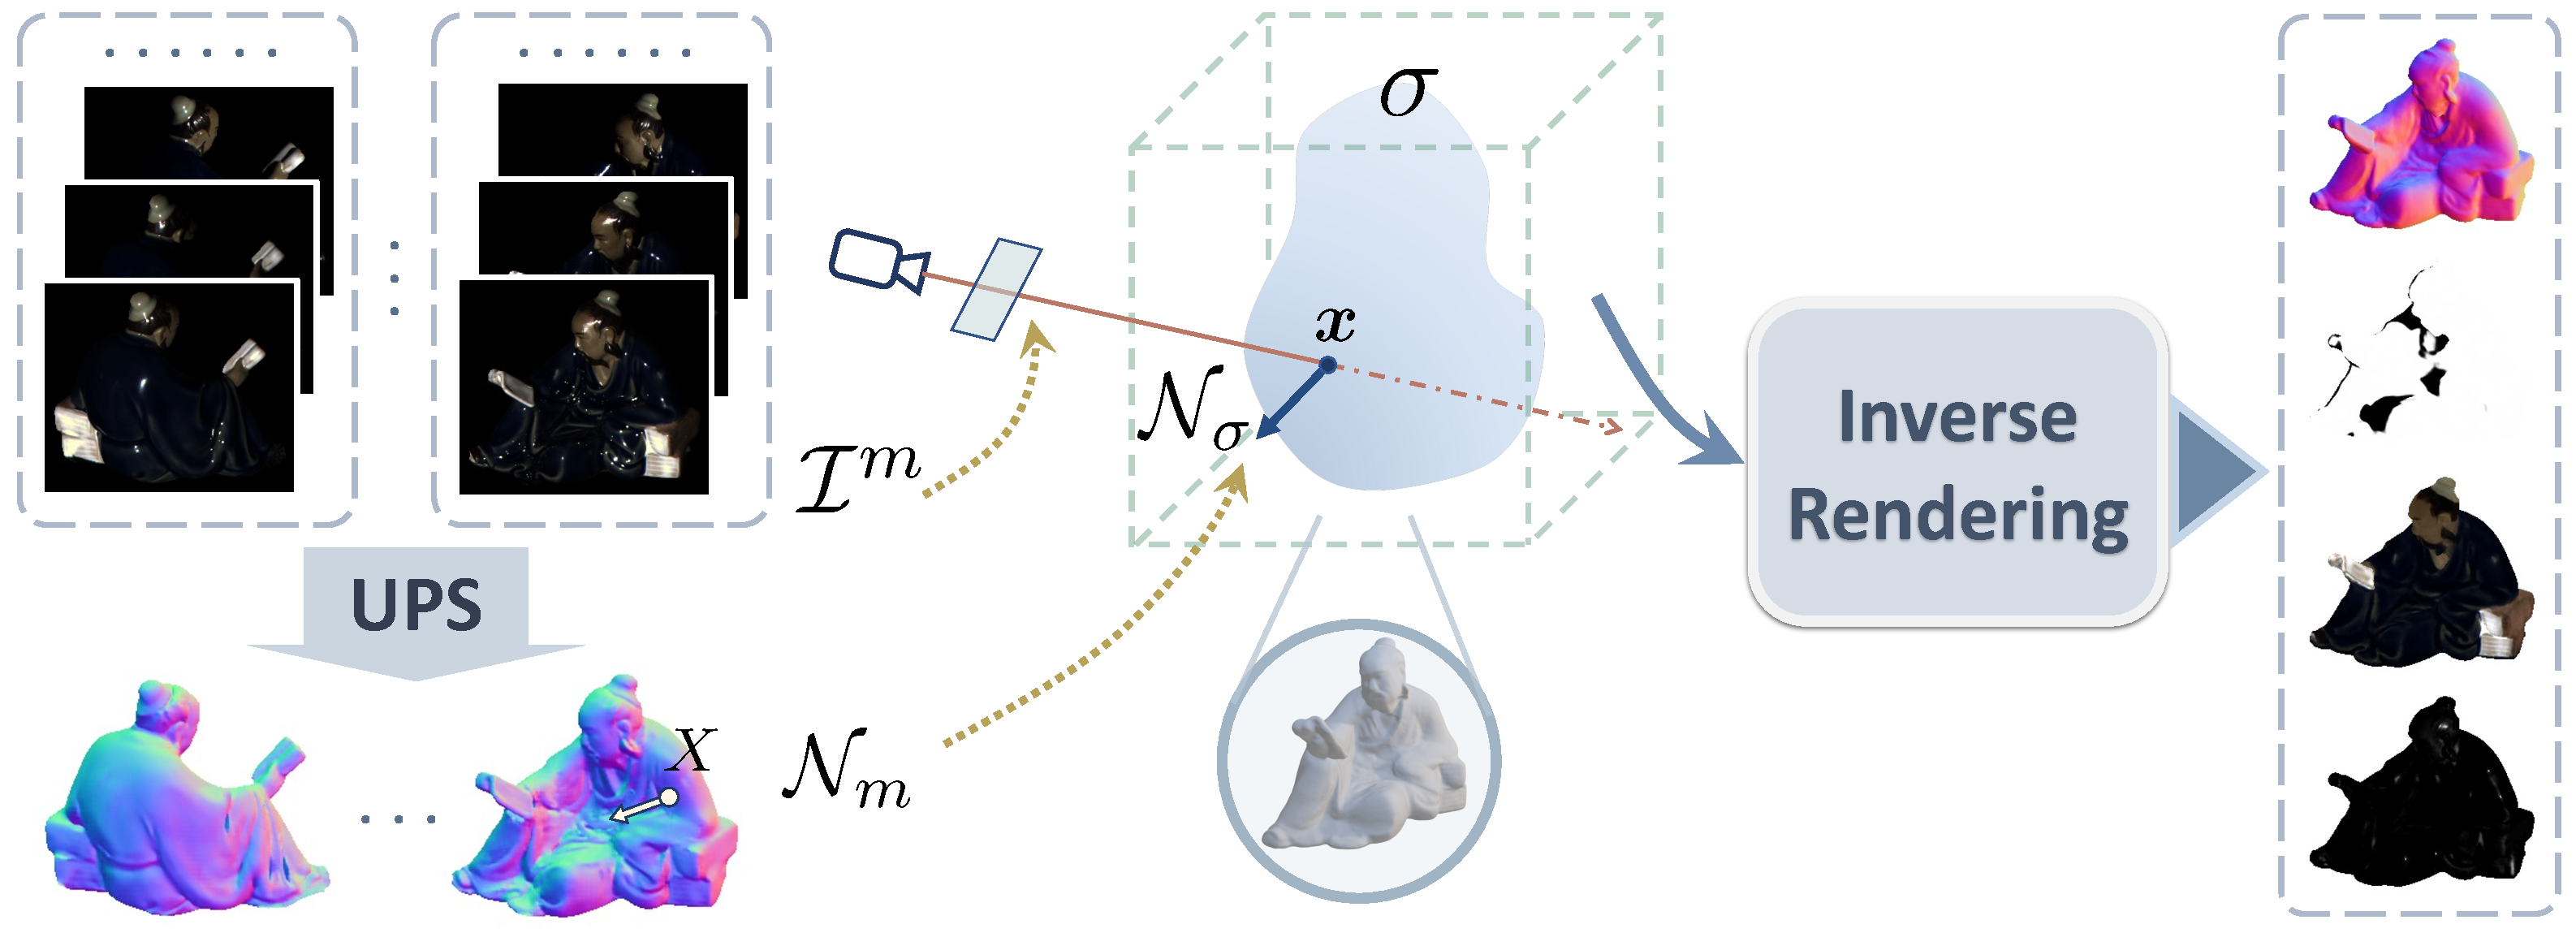
\includegraphics[width=0.95\textwidth]{images/overall_v2.pdf}
    \end{center}
    \vspace{-0.8em}
    \textbf{\color{ctitle}Stage I -- Initial Shape Modeling:} \\
    We estimate a guidance normal map $\mathcal{N}_{m}$ for each view, which is used to supervise the normals derived from the density field. This direct normal supervision is expected to provide a strong regularization on the density field, leading to an accurate surface. 
    \vspace{-0.5em}
    \begin{center}
        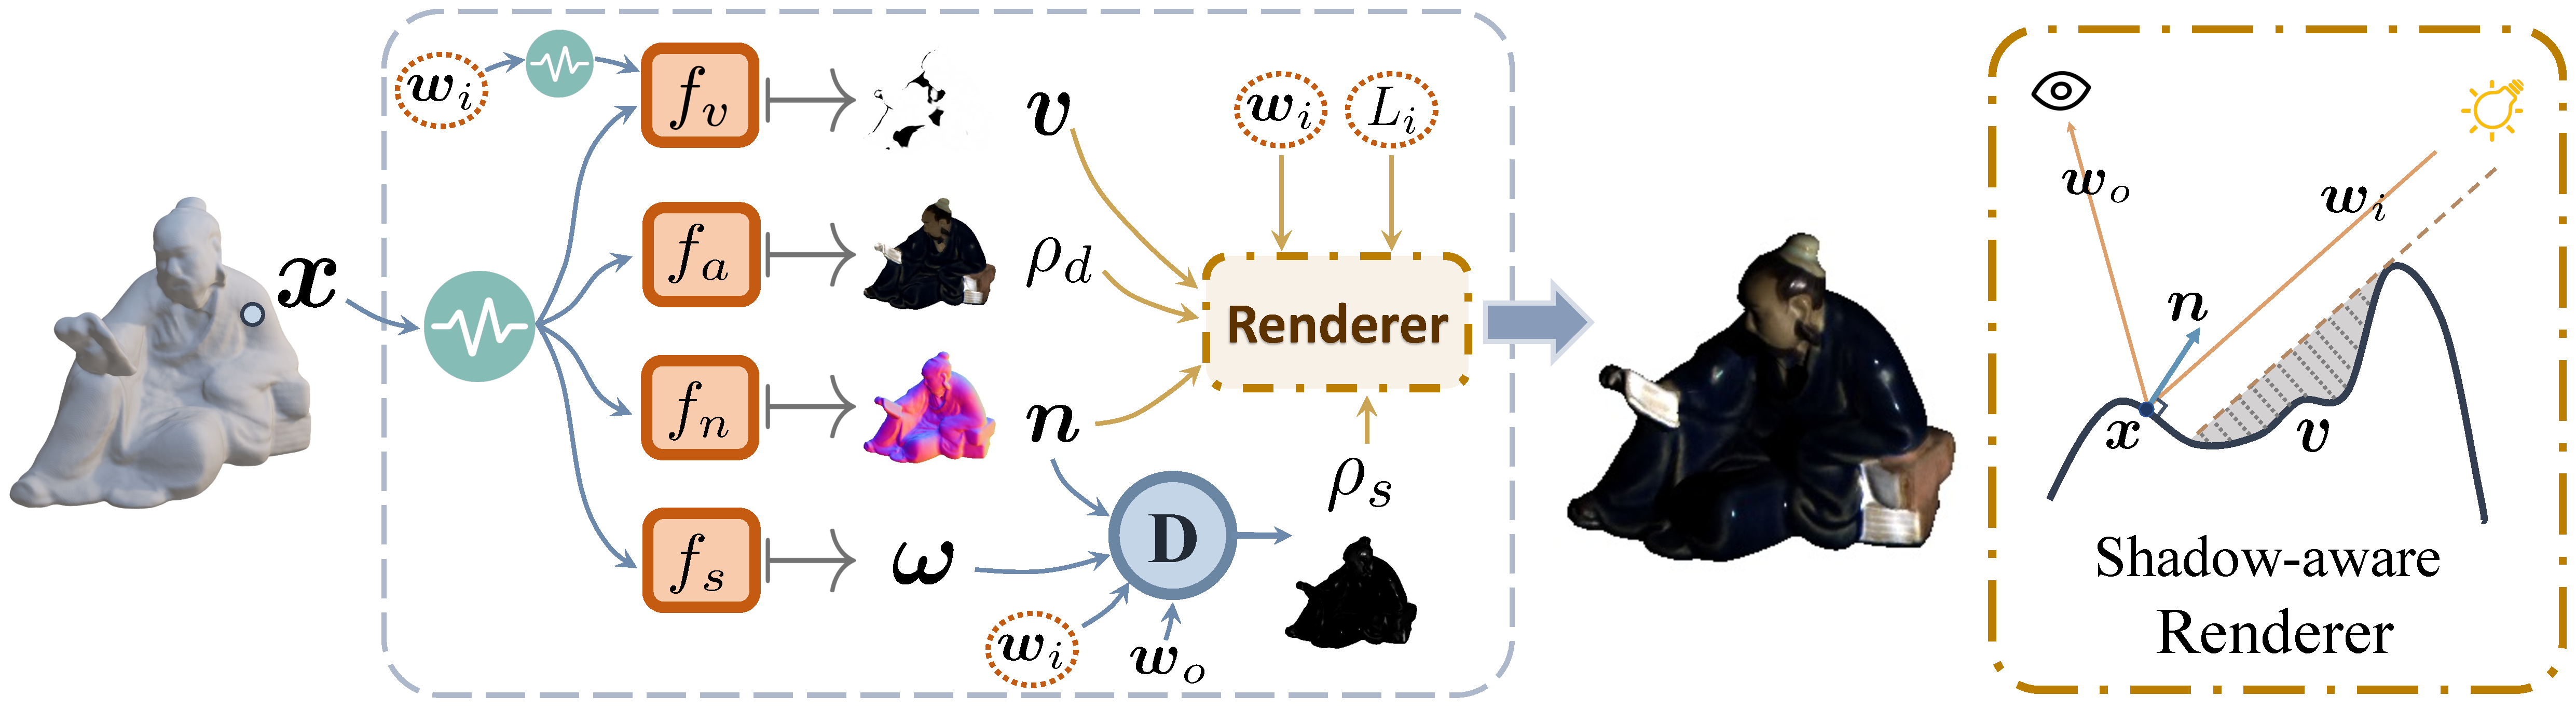
\includegraphics[width=0.95\textwidth]{images/stage2_v2.pdf}
    \end{center}
    \vspace{-0.6em}
    \textbf{\color{ctitle}Stage II -- Joint Optimization with Inverse Rendering:}  \\
    Based on the learned density field as the shape prior, we jointly optimize the surface normals, materials, and lights using a shadow-aware rendering layer. 
    \begin{itemize}
        \item We model normals, BRDFs, and light visibility with MLPs. The weights of the MLPs and lights are jointly optimized to fit the input images.
        \item The rendering equation with directional light and visibility is:
    \end{itemize}
    \vspace{-0.7em}
    \begin{align*}
        \lout (\dout,\din; \point) = \vmlp (\din; \point) \lin (\din) \brdf (\dout, \din; \point) (\din \cdot \normal).
    \end{align*}
}
%
\headerbox{\bf\color{ctitle} Experiments \& Results}{name=results,column=2,below=contribution,span=4}{
    \begin{minipage}[t]{0.49\textwidth}
        %%%%%%%%%%%%%%%%%%%%%%%% MVPS  %%%%%%%%%%%%%%%%%%%%%%%%%%%%%
        \textbf{\color{ctitle}Comparison with MVPS Methods:}
        %%%%%%%%%%%%%%%%%%%%%%%% table  %%%%%%%%%%%%%%%%%%%%%%%%%%%%%
        % \vspace{0.2em}
        \vspace{-0.6em}
        \begin{center}
            Quantitative results on DiLiGenT-MV benchmark \\
            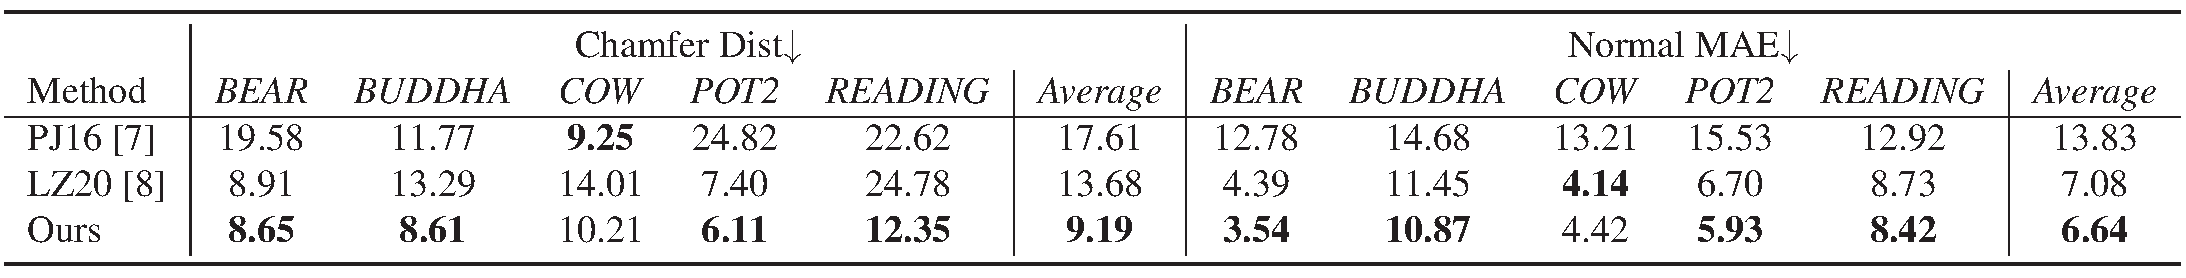
\includegraphics[width=\textwidth]{images/table_ps.pdf}
        \end{center}
        \vspace{-2em}
        %%%%%%%%%%%%%%%%%%%%%%%% figure  %%%%%%%%%%%%%%%%%%%%%%%%%%%%%
        \begin{center}
            Qualitative results of shape and normal on DiLiGenT-MV benchmark \\
            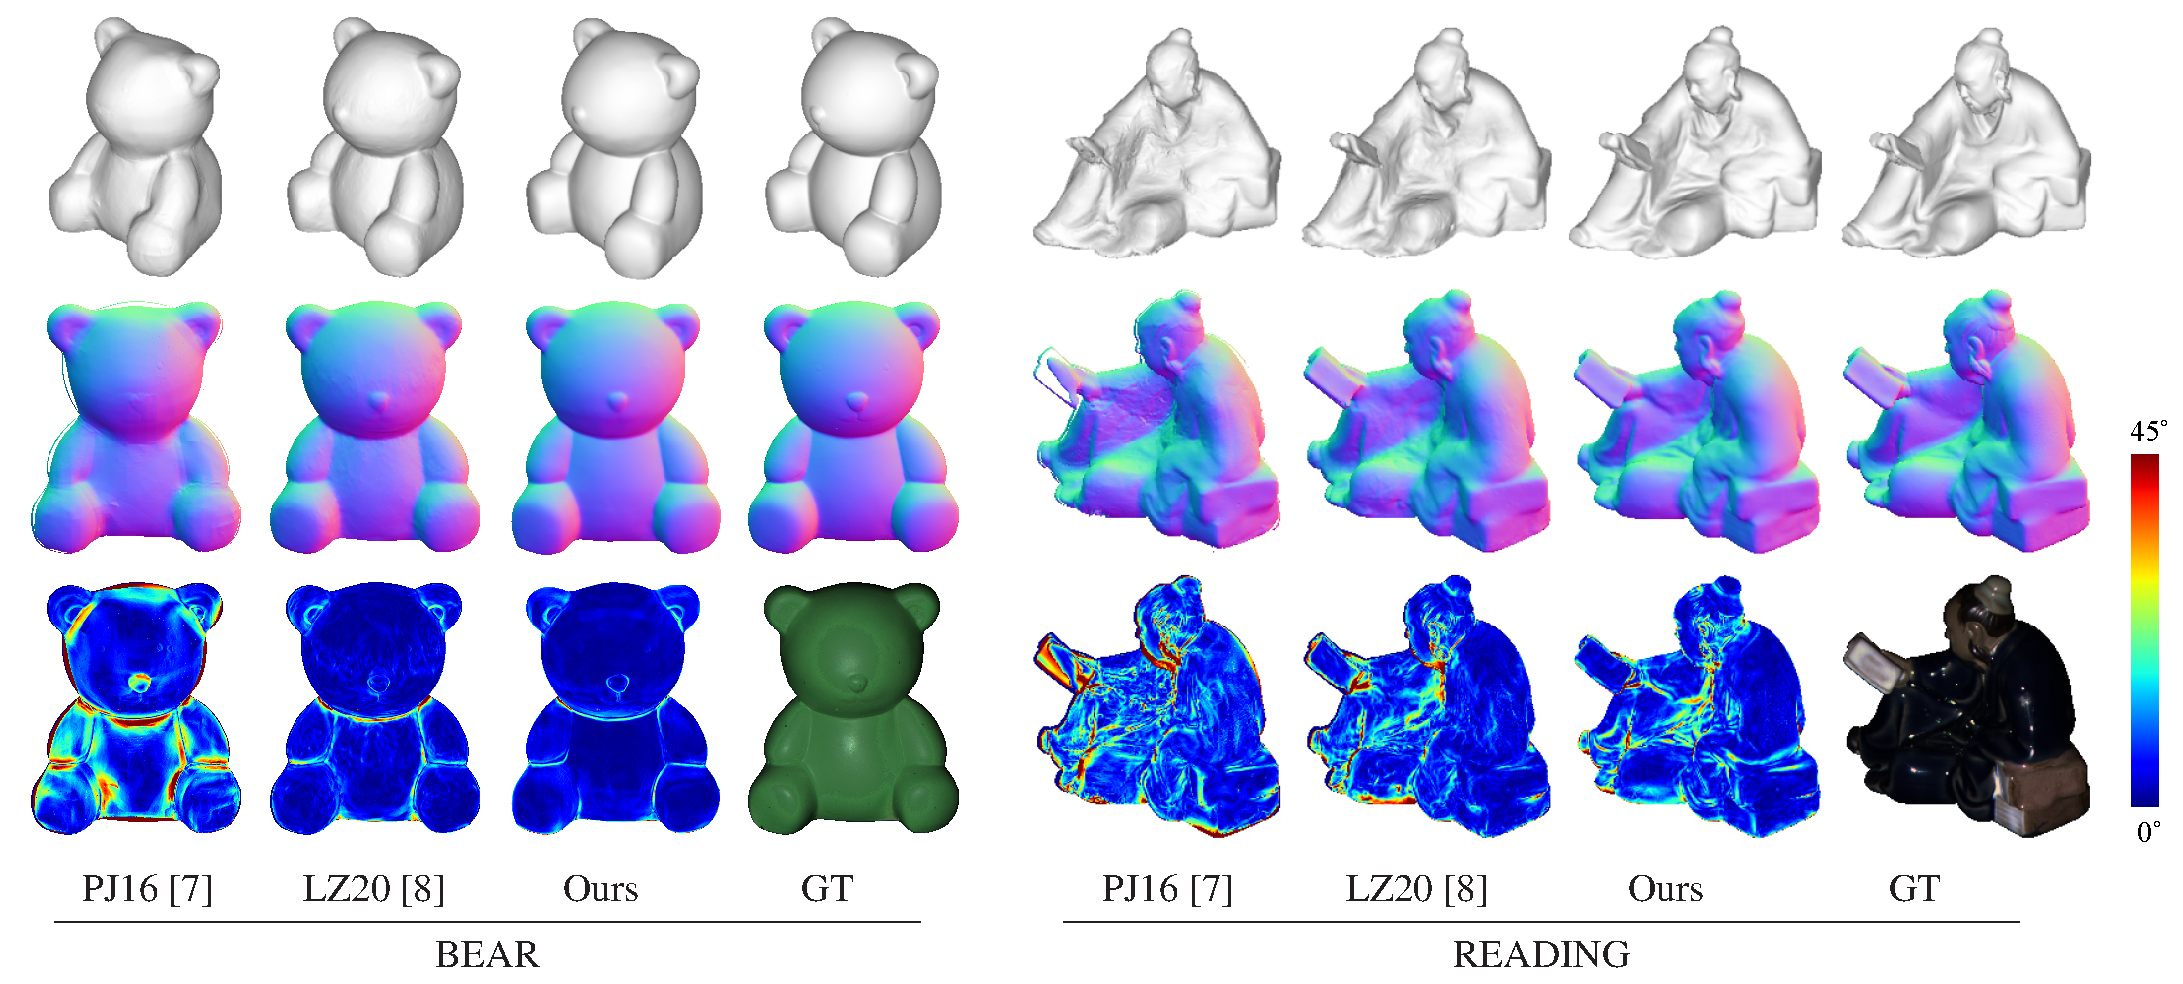
\includegraphics[width=\textwidth]{images/fig_ps.pdf}
        \end{center}
        
        %%%%%%%%%%%%%%%%%%%%%%%% NORMAL REG  %%%%%%%%%%%%%%%%%%%%%%%%%%%%%
        \vspace{-0.5em}
        \textbf{\color{ctitle}Effectiveness of Normal Regularization:}
        %%%%%%%%%%%%%%%%%%%%%%%% table  %%%%%%%%%%%%%%%%%%%%%%%%%%%%%
        % \vspace{0.2em}
        \vspace{-0.6em}
        \begin{center}
            Quantitative analysis on normal supervision \\
            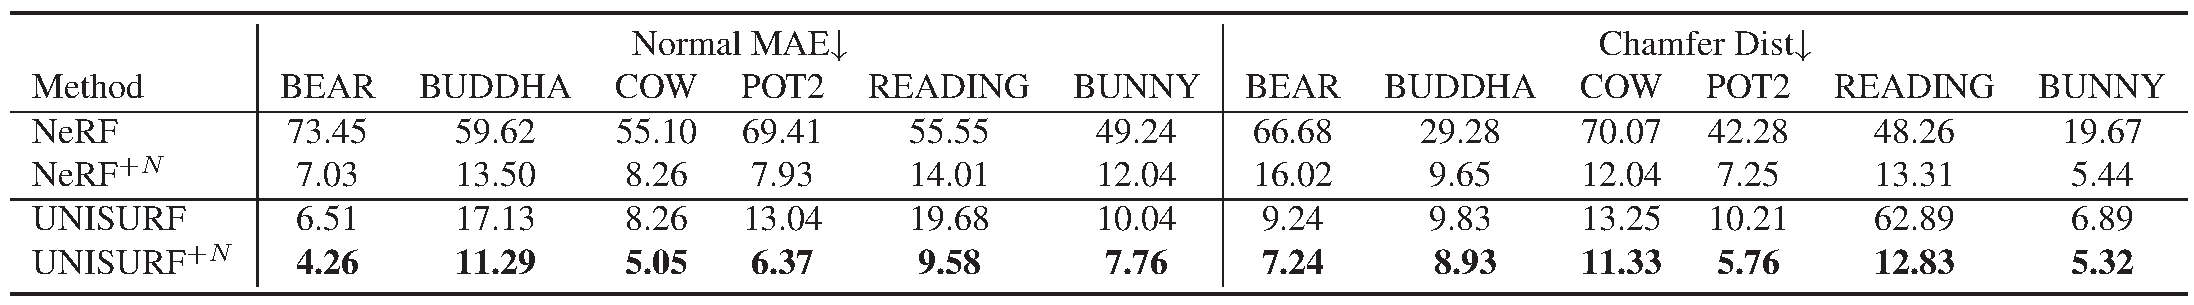
\includegraphics[width=\textwidth]{images/table_analysis_normal.pdf}
        \end{center}
        \vspace{-1.8em}
        %%%%%%%%%%%%%%%%%%%%%%%% figure  %%%%%%%%%%%%%%%%%%%%%%%%%%%%%
        \begin{center}
            Qualitative comparison on w/ \& w/o normal supervision \\[0.2em]
            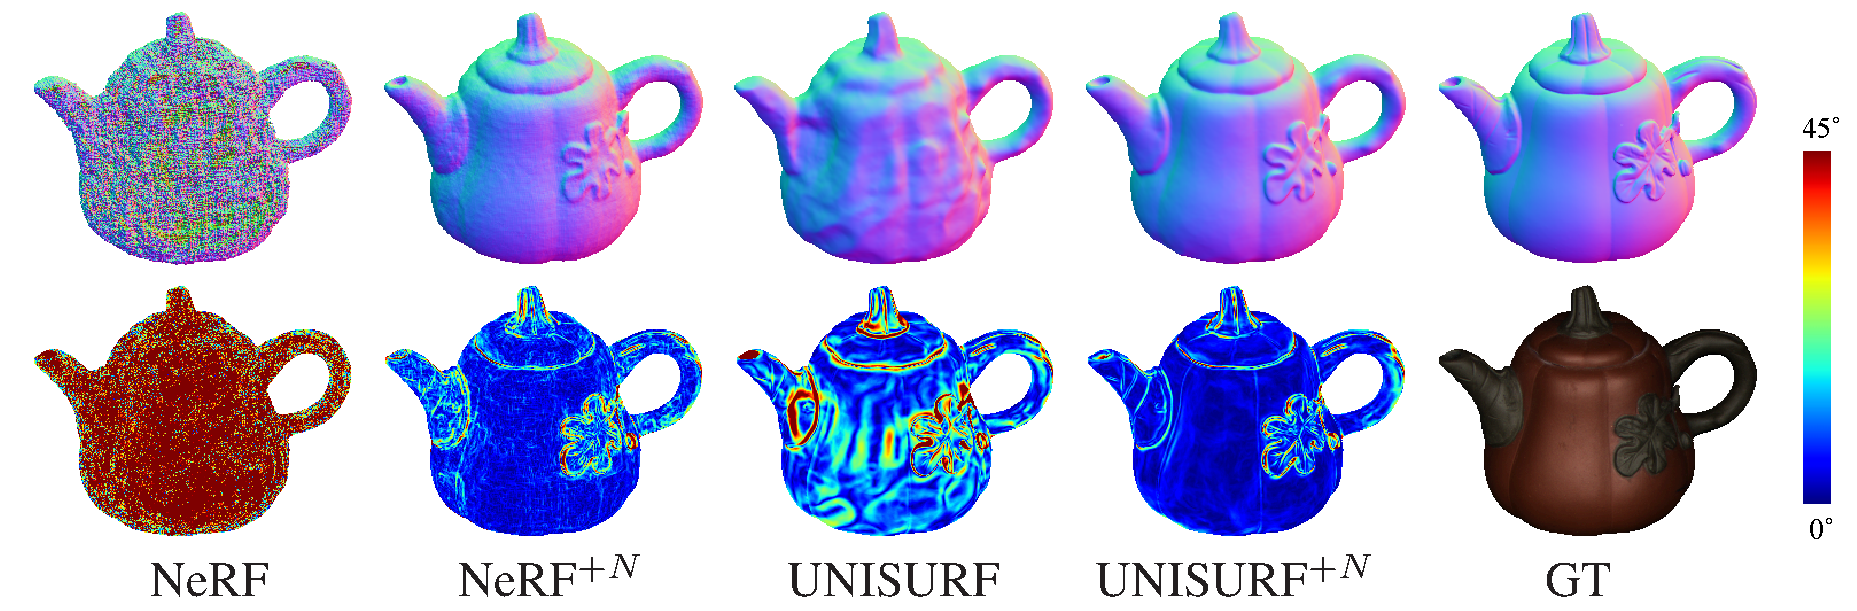
\includegraphics[width=0.8\textwidth]{images/fig_analysis_normal.pdf}
        \end{center}
    \end{minipage}\hfill
    %%%%%%%%%%%%%%%%%%%%%%%%%%%%%%%%%%%%%%%%%%%%%%%%%%%%%%%%%%%%%%%%%%
    %%%%%%%%%%%%%%%%% second column %%%%%%%%%%%%%%%%%%%%%%%%%%%%%%%%%%
    %%%%%%%%%%%%%%%%%%%%%%%%%%%%%%%%%%%%%%%%%%%%%%%%%%%%%%%%%%%%%%%%%%
    \begin{minipage}[t]{0.49\textwidth}
        %%%%%%%%%%%%%%%%%%%%%%%% NRF  %%%%%%%%%%%%%%%%%%%%%%%%%%%%%
        \textbf{\color{ctitle}Comparison with Neural Rendering Based Methods:} 
        %%%%%%%%%%%%%%%%%%%%%%%% table  %%%%%%%%%%%%%%%%%%%%%%%%%%%%%
        % \vspace{0.2em}
        \vspace{-0.6em}
        \begin{center}
            Comparison of shape reconstruction results on real and synthetic datasets \\
            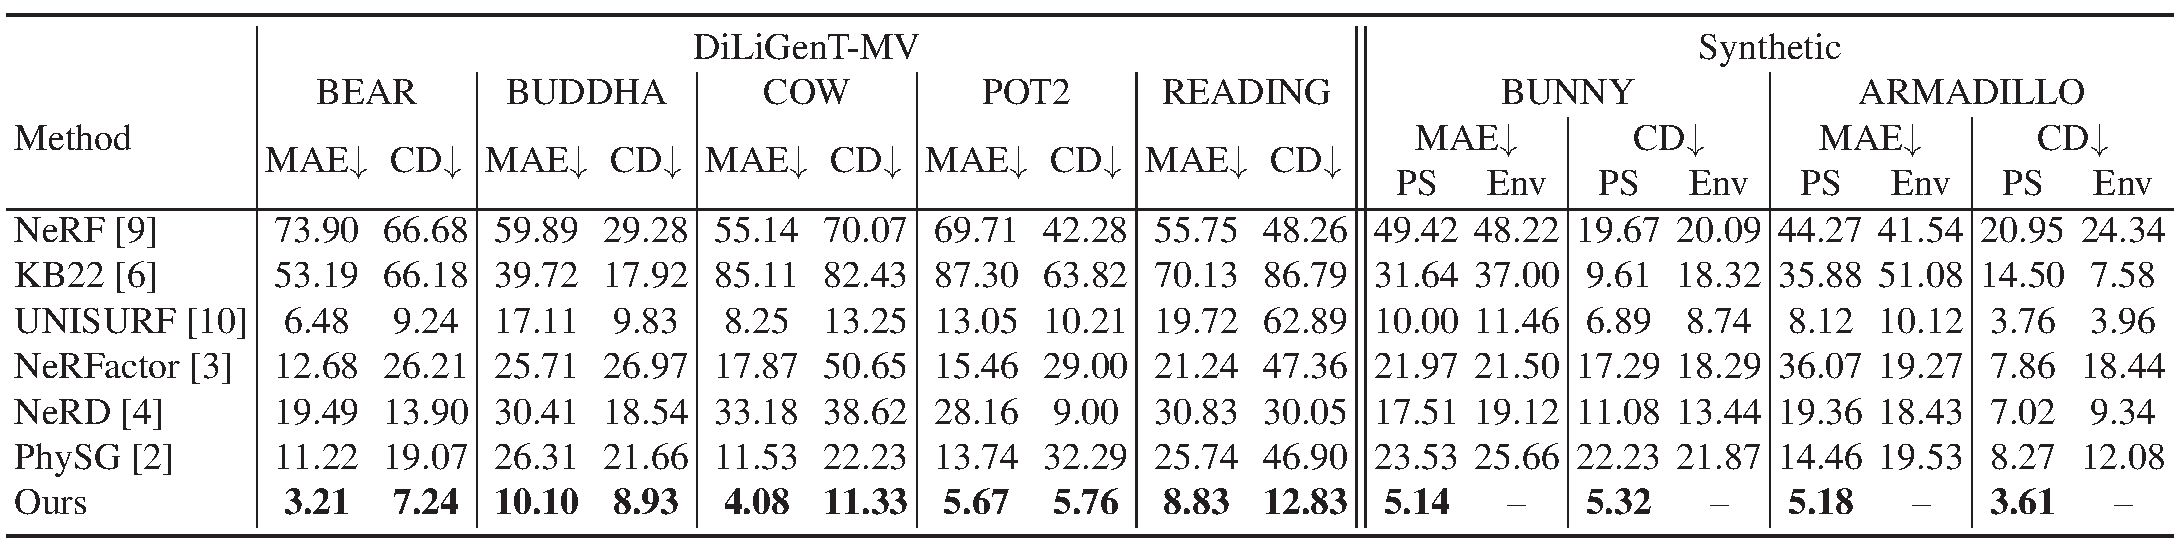
\includegraphics[width=\textwidth]{images/table_nrf.pdf}
        \end{center}
        \vspace{-2em}
        %%%%%%%%%%%%%%%%%%%%%%%% figure  %%%%%%%%%%%%%%%%%%%%%%%%%%%%%
        \begin{center}
            Novel view rendering and normal estimation results on the synthetic dataset  \\
            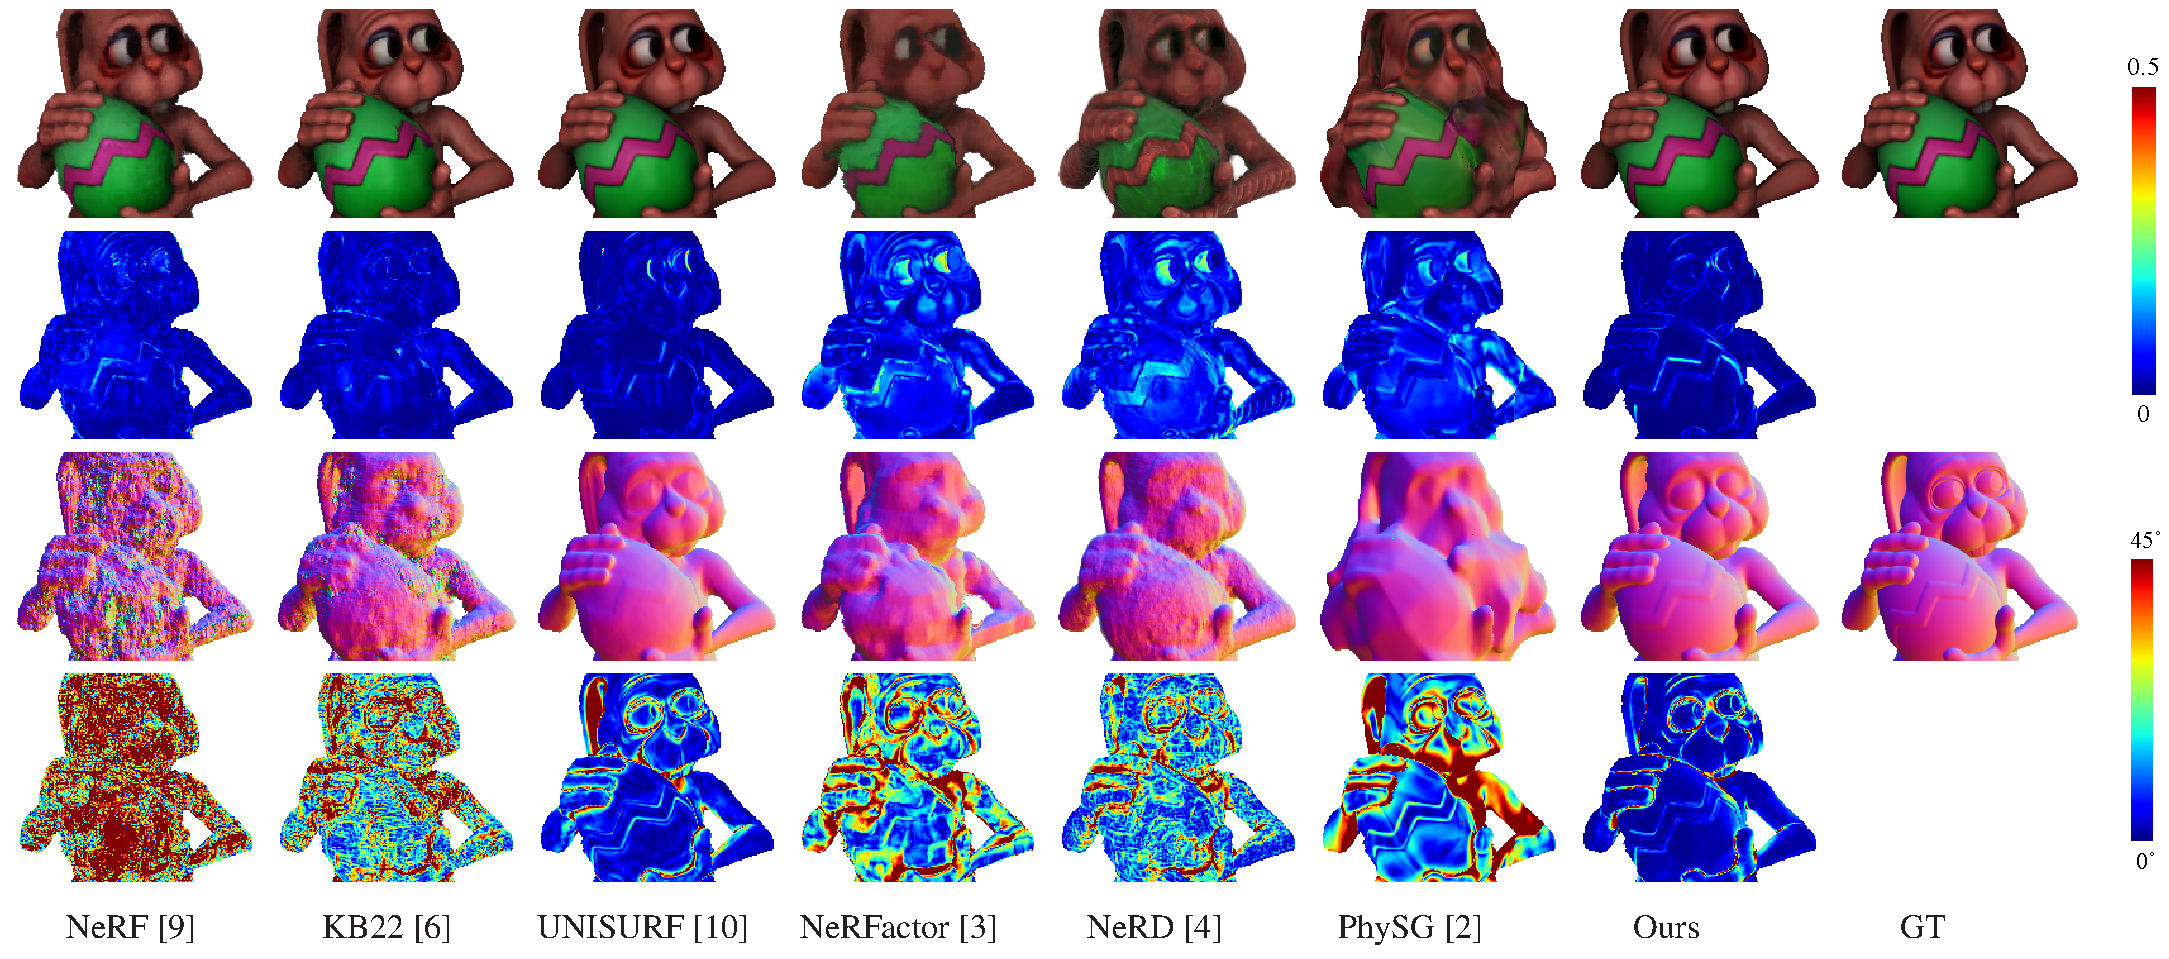
\includegraphics[width=0.96\textwidth]{images/fig_nrf.pdf}
        \end{center}
        
        \vspace{-0.5em}
        %%%%%%%%%%%%%%%%%%%%%%%% IMPROVEMENT  %%%%%%%%%%%%%%%%%%%%%%%%%%%%%
        \begin{minipage}[t]{0.53\textwidth}
        \textbf{\color{ctitle}Normal Improvement:} \\
            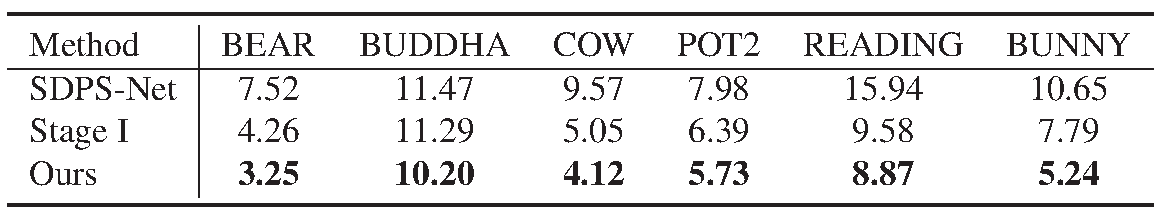
\includegraphics[width=\textwidth]{images/table_improve_normal.pdf}
        
        \textbf{\color{ctitle}Light Improvement:} \\
            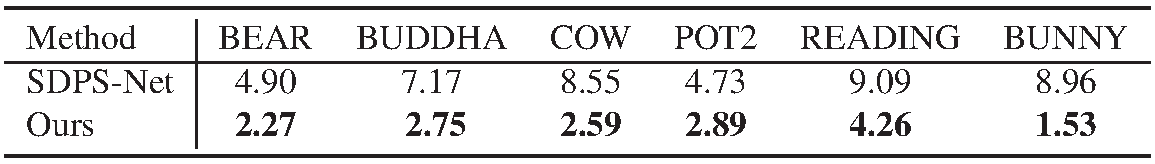
\includegraphics[width=\textwidth]{images/table_improve_light.pdf}
        \end{minipage}\hfill
        %%%%%%%%%%%%%%%%%%%%%%%% APPLICATION V2  %%%%%%%%%%%%%%%%%%%%%%%%%%%%%
        \begin{minipage}[t]{0.465\textwidth}
            \textbf{\color{ctitle}Decomposition and Applications:}
            %%%%%%%%%%%%%%%%%%%%%%%% figure  %%%%%%%%%%%%%%%%%%%%%%%%%%%%%
            \vspace{-2em}
            \begin{center} 
                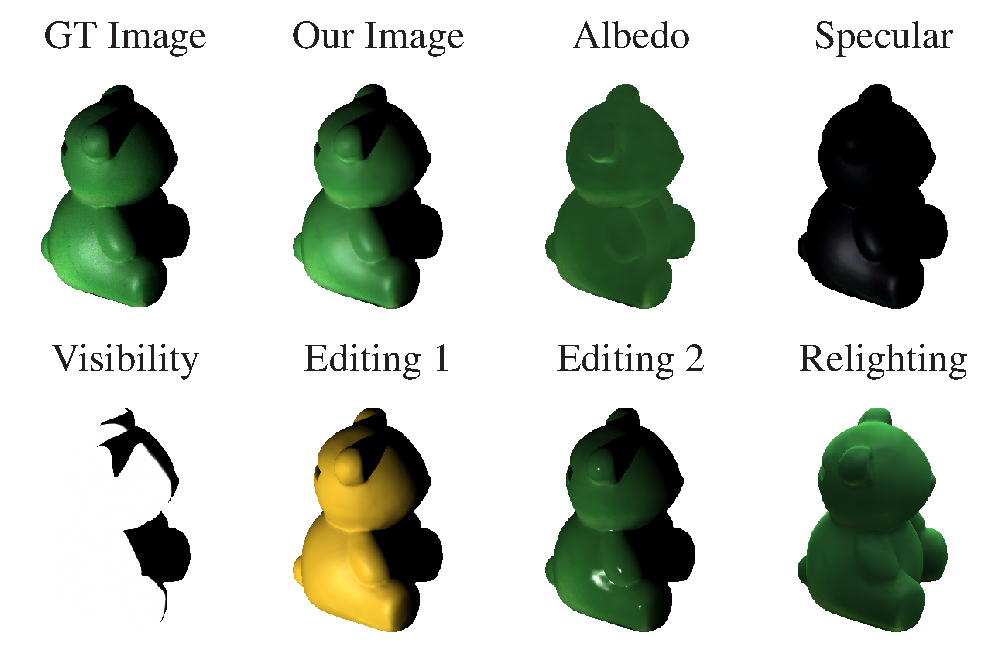
\includegraphics[width=0.96\textwidth]{images/fig_application.pdf}
            \end{center}
        \end{minipage}
        
        %%%%%%%%%%%%%%%%%%%%%%%% REFERENCE  %%%%%%%%%%%%%%%%%%%%%%%%%%%%%
        \vspace{-1em}
        \textbf{\color{ctitle}References:} \\
        \begin{minipage}[t]{0.25\textwidth}
            \vspace{-0.5em}
            \begin{enumerate}[label={[\arabic*]}, leftmargin=*]
                \scriptsize
                \item NeRV [Srinivasan~\emph{et al.}, CVPR21]
                \item PhySG [Zhang~\emph{et al.}, CVPR21]
            \end{enumerate}
        \end{minipage}\hfill
        \begin{minipage}[t]{0.36\textwidth}
            \vspace{-0.5em}
            \begin{enumerate}[label={[\arabic*]}, leftmargin=*]
                \scriptsize
                \setcounter{enumi}{2}
                \item NeRFactor [Zhang~\emph{et al.}, TOG21]
                \item NeRD [Boss~\emph{et al.}, ICCV21]
                \item NRF [Bi~\emph{et al.}, arXiv20]
                \item KB22 [Kaya~\emph{et al.}, WACV22]
            \end{enumerate}
        \end{minipage}\hfill
        \begin{minipage}[t]{0.38\textwidth}
            \vspace{-0.5em}
            \begin{enumerate}[label={[\arabic*]}, leftmargin=*]
                \scriptsize
                \setcounter{enumi}{6}
                \item PJ16 [Park~\emph{et al.}, TPAMI16]
                \item LZ20 [Li~\emph{et al.}, TIP20]
                \item NeRF [Mildenhall~\emph{et al.}, ECCV20]
                \item UNISURF [Oechsle~\emph{et al.}, ICCV21]
            \end{enumerate}
        \end{minipage}
    \end{minipage}

}
\end{poster}
\end{document}